\documentclass[11pt]{article}
\usepackage{graphicx}
\usepackage{epstopdf} 
\begin{document}
\begin{titlepage}
%\selectlanguage{english}

%----------------------------------------------------------------------------------------
% TITLE PAGE INFORMATION
%----------------------------------------------------------------------------------------
  \begin{center} % Center everything on the page

  %----------------------------------------------------------------------------------------
  % HEADING SECTIONS
  %----------------------------------------------------------------------------------------
  \textsc{\large Facultatea Calculatoare, Informatica si Microelectronica}\\[0.5cm]
  \textsc{\large Universitatea Tehnica a Moldovei}\\[1.2cm] % Name of your university/college
  \vspace{25 mm}

  \textsc{\Large Medii Interactive de Dezvoltare a Produselor Soft}\\[0.5cm] % Major heading such as course name
  \textsc{\large Lucrarea de laborator\#3}\\[0.5cm] % Minor heading such as course title
  %\textsc{\large Laboratory work}\\[0.5cm] % Minor heading such as course title

\newcommand{\HRule}{\rule{\linewidth}{0.5mm}} % Defines a new command for the horizontal lines, change thickness here

  %----------------------------------------------------------------------------------------
  % TITLE SECTION
  %----------------------------------------------------------------------------------------
  \vspace{10 mm}
  \HRule \\[0.4cm]
  { \LARGE \bfseries Web development  }\\[0.4cm] % Title of your document
  \HRule \\[1.5cm]

  %----------------------------------------------------------------------------------------
  % AUTHOR SECTION
  %----------------------------------------------------------------------------------------
      \vspace{30mm}

      \begin{minipage}{0.4\textwidth}
      \begin{flushleft} \large
      \emph{Autor:}\\
      Cristina \textsc{Bradu}
      \end{flushleft}
      \end{minipage}
      ~
      \begin{minipage}{0.4\textwidth}
      \begin{flushright} \large
      \emph{lector asistent:} \\
      Irina \textsc{Cojanu} \\ % Supervisor's Name 
      \emph{lector superior:} \\
      Radu \textsc{Melnic} % Supervisor's Name
      \end{flushright}
      \end{minipage}\\[4cm]

      \vspace{5 mm}
      % If you don't want a supervisor, uncomment the two lines below and remove the section above
      %\Large \emph{Author:}\\
      %John \textsc{Smith}\\[3cm] % Your name

      %----------------------------------------------------------------------------------------
      % DATE SECTION
      %----------------------------------------------------------------------------------------

      %{\large \today}\\[3cm] % Date, change the \today to a set date if you want to be precise

      %----------------------------------------------------------------------------------------
      % LOGO SECTION
      %----------------------------------------------------------------------------------------

      %\includegraphics{red}\\[0.5cm] % Include a department/university logo - this will require the graphicx package

      %----------------------------------------------------------------------------------------

      \vfill % Fill the rest of the page with whitespace
      \end{center}
      
\end{titlepage}

\begin{LARGE}
\textit{Lucrarea de laborator nr.3}
\end{LARGE}

\section{Scopul lucrarii de laborator}

Studierea si implementarea cunostintelor in Web Development

\section{Obiective}

Realizarea unui simplu Web Site personal, a unui mockup corespunzatorul site-ului care urmeaza a fi realizat, familiarizarea cu HTML si CSS, interactiuni Javascript

\section{Analiza lucrarii de laborator}

\subsection{Cerintele implementate}

Realizeaza un mini site cu 3 pagini statice
Site-ul trebuie sa pastreze toata informatia intr-o baza de date
Site-ul trebuie sa contina AJAX Requests.
Implimentarea XHR sau JSON responses. Unele informatii trebuie sa fie dinamic incarcata pe pagina


\subsection{Continutul lucrarii}
Link-ul repozitoriului: 
\begin{center}
\textbf{https://github.com/BraduCristina/MIDPS}
\end{center}

In lucrarea de laborator nr.3, am facut cunostinta cu Web Development - Dezvoltarea Web.
Pentru a indeplini sarcina propusa la inceputul lucrarii, am studiat, si ulterior, am implementat, asa tehnologii, ca
HTML/CSS, am lucrat cu bazele de date PHP si MySQL, dar si am operat cu Request-urile AJAX is am implementat JSON responses.
Am optat pentru crearea unei pagini web pentru un restaurant, ce vizeaza date despre  acest restaurant, contactele administratiei si localizarea sa pe harta, utilizind tehnologiile Google Maps, la fel am lucrat si cu Javascript-ul si Jquery.
Aceste tehnologii m-au ajutat sa incarc informatia dinamic pe site si sa fac site-ul cit mai atragator pentru utilizator.
Am prevazut si crearea unei forme de inregistrare pe site, utilizind MySQL si PHP, pentru ca administratorul sa poata stoca datele referitor la dinamica site-ului, accesibilitatea informatiei, dar si popularitatea restaurantului.
Utilizind instrumentele jquery am facut in asa mod, ca pagina de baza al site-ului sa fie o imagine fullscreen, ceea ce capteaza atentia utilizatorului, tehnici intilnite de mine la multe site-uri destul de populare.
La fel, asa cum ne aflam in era inaltelor si dinamicelor dezvoltari, am prevazut si navigarea pe site de pe orice dispozitiv "smart". Am creat un site adaptiv pentru orice dimensiuni, astfel ca utilizatorul sa nu fie intimidat de modul in care se afiseaza informatia, indiferent de pe care dispozitiv acesta o acceseaza.
Mai jos, anexez screen-shot-uri cu site-ul in general si vizualizarea lui pe smartphone-uri si tablete.

%--------------------------------------------------
\section{Anexa 1 (figures)}
%--------------------------------------------------

\begin{figure}[h]

\includegraphics{images/1.eps}
\caption{Pagina principala - main}
\end{figure}

\begin{figure}[h]
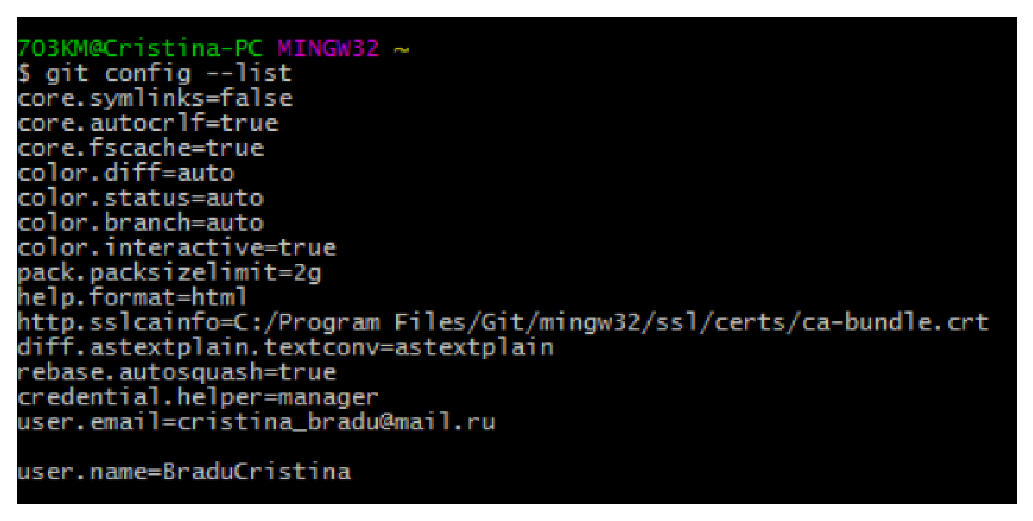
\includegraphics{images/2.eps}
\caption{Pagina Home (Acasa)}
\end{figure}

\begin{figure}[h]

\includegraphics{images/21.eps}
\caption{Pagina Home (Acasa)}
\end{figure}

\begin{figure}[h]
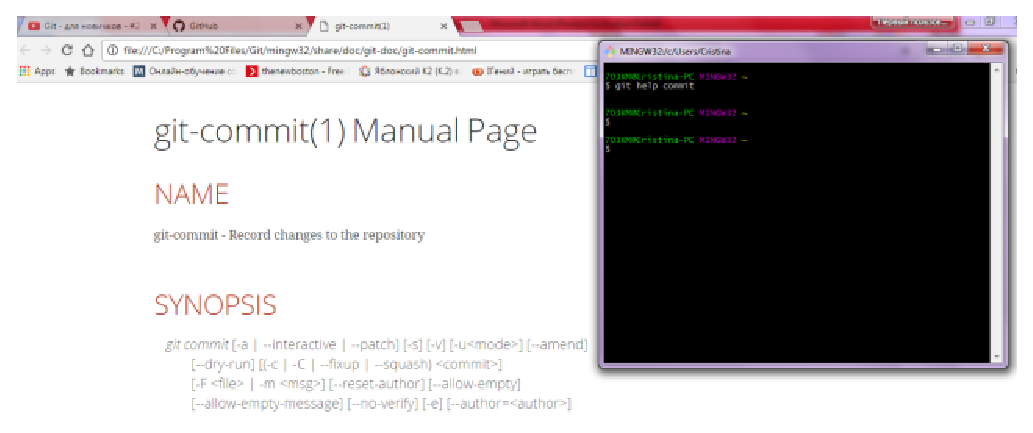
\includegraphics{images/3.eps}
\caption{Pagina About Us (Despre Noi)}
\end{figure}

\begin{figure}[h]
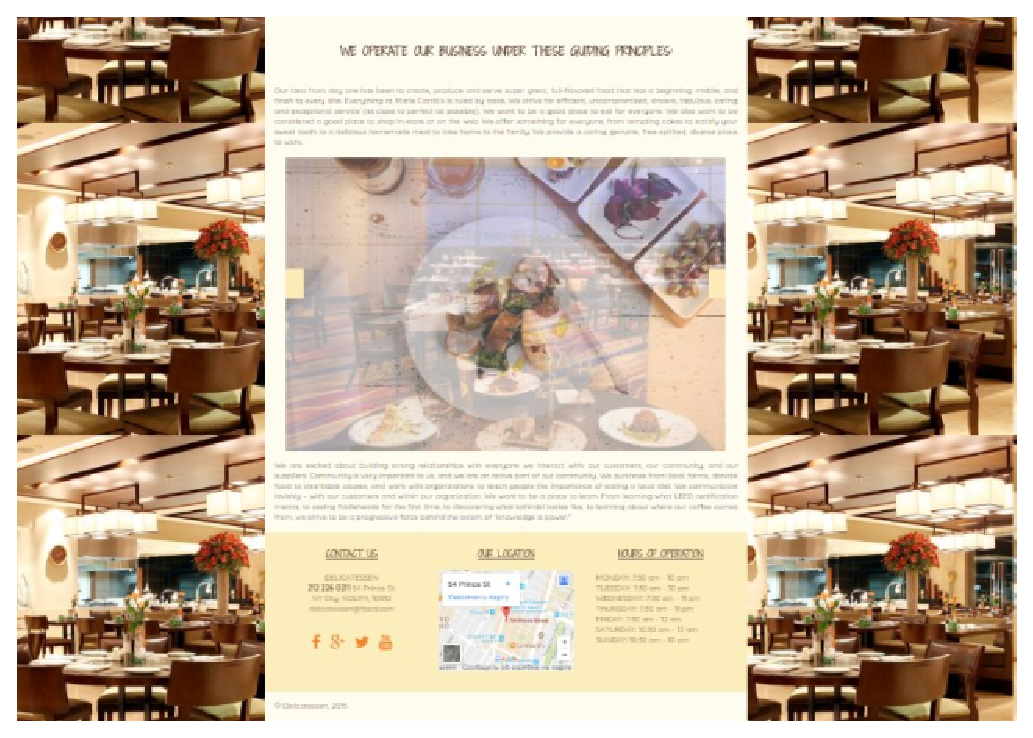
\includegraphics{images/31.eps}
\caption{Pagina About Us (Despre Noi)}
\end{figure}

\begin{figure}[h]
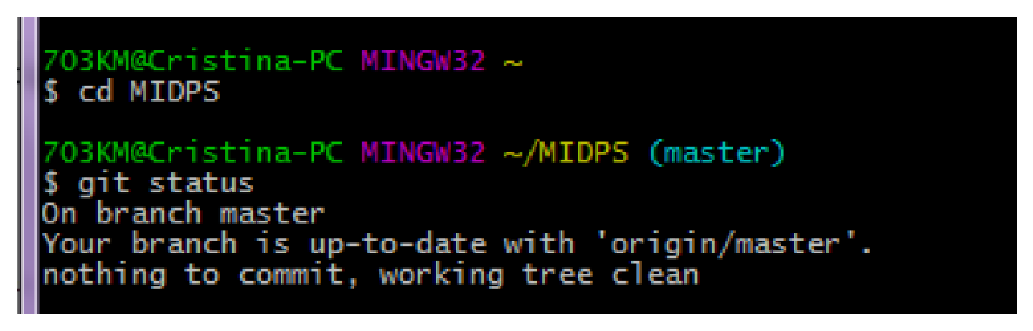
\includegraphics{images/4.eps}
\caption{Pagina Contact (Contacteaza-ne)}
\end{figure}

\begin{figure}[h]

\includegraphics{images/5.eps}
\caption{Pagina Gallery (Galerie Foto)}
\end{figure}

\begin{figure}[h]
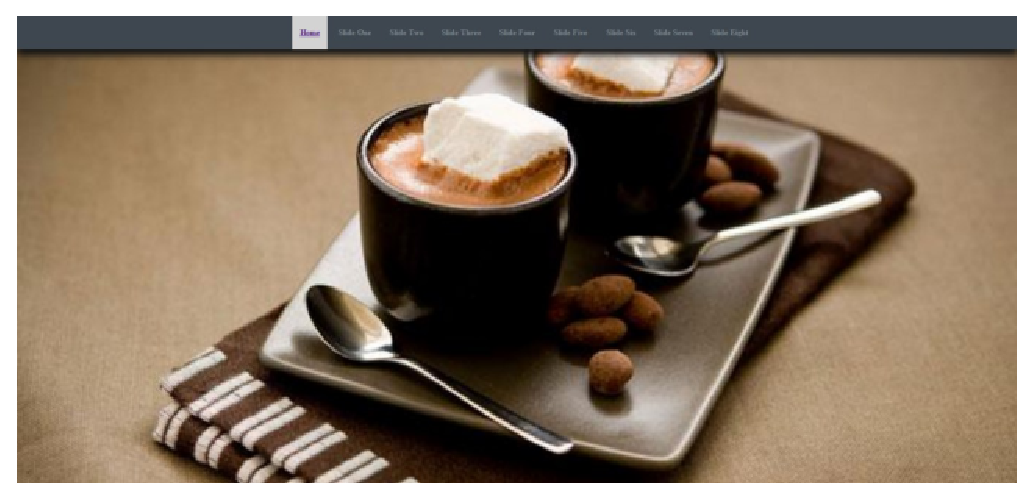
\includegraphics{images/51.eps}
\caption{Pagina Gallery (Galerie Foto)}
\end{figure}

\begin{figure}[h]

\includegraphics{images/52.eps}
\caption{Pagina Gallery (Galerie Foto)}
\end{figure}

\begin{figure}[h]
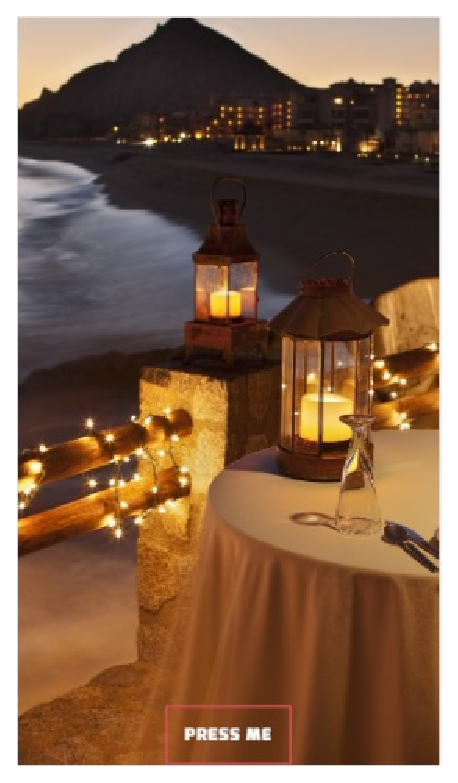
\includegraphics{images/6.eps}
\caption{Afisare Smartphone - main}
\end{figure}

\begin{figure}[h]

\includegraphics{images/7.eps}
\caption{Afisare Smartphone - Home}
\end{figure}

\begin{figure}[h]
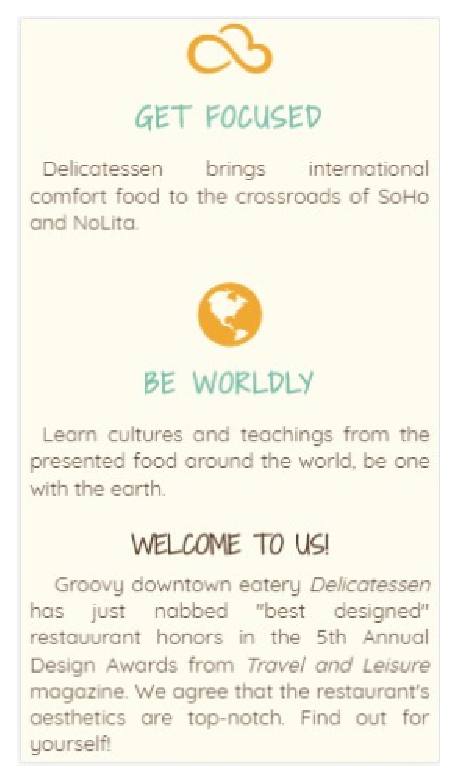
\includegraphics{images/71.eps}
\caption{Afisare Smartphone - Home}
\end{figure}\

\begin{figure}[h]
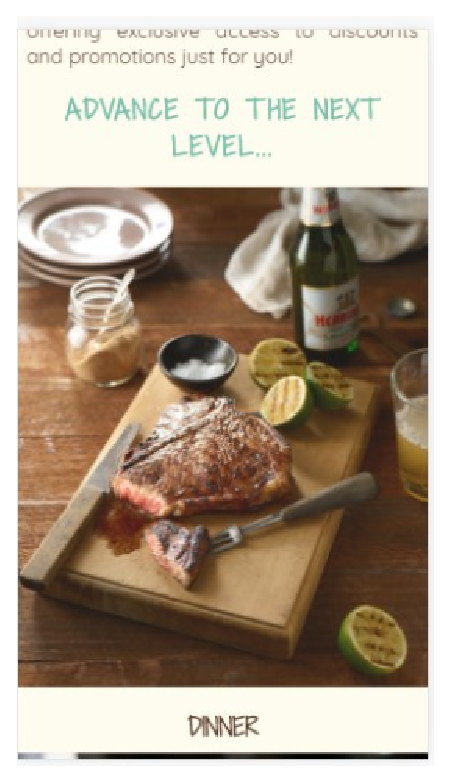
\includegraphics{images/72.eps}
\caption{Afisare Smartphone - Home}
\end{figure}

\begin{figure}[h]
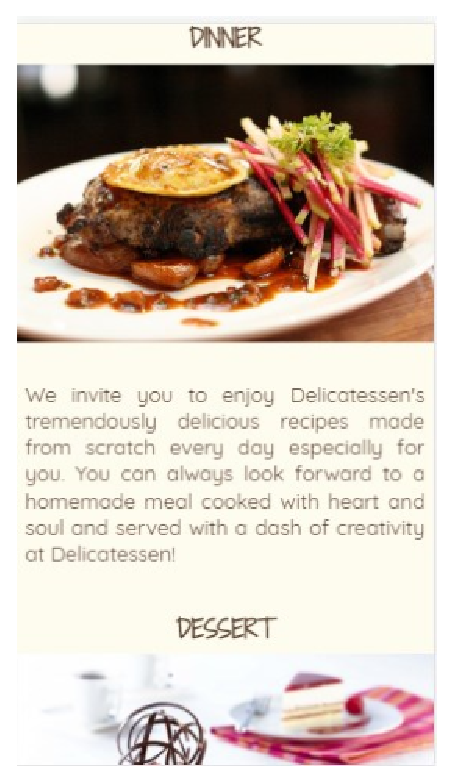
\includegraphics{images/73.eps}
\caption{Afisare Smartphone - Home}
\end{figure}

\begin{figure}[h]
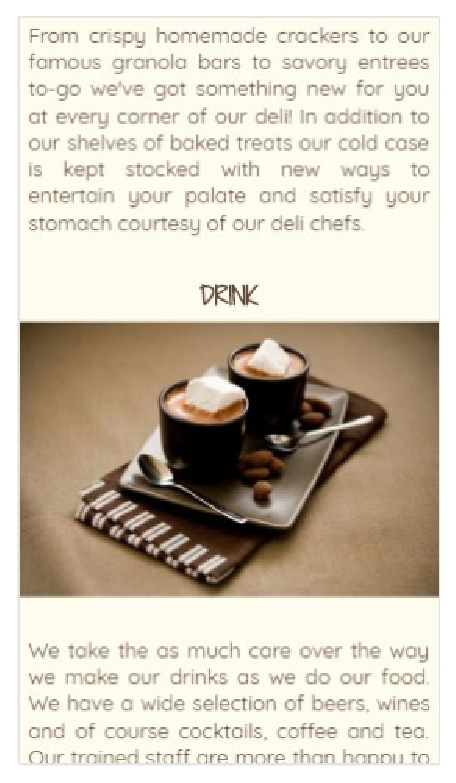
\includegraphics{images/74.eps}
\caption{Afisare Smartphone - Home}
\end{figure}

\begin{figure}[h]
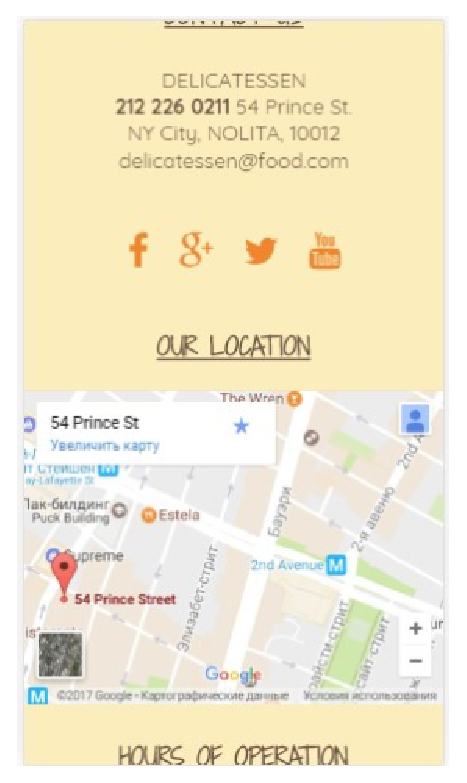
\includegraphics{images/75.eps}
\caption{Afisare Smartphone - Home}
\end{figure}

\begin{figure}[h]
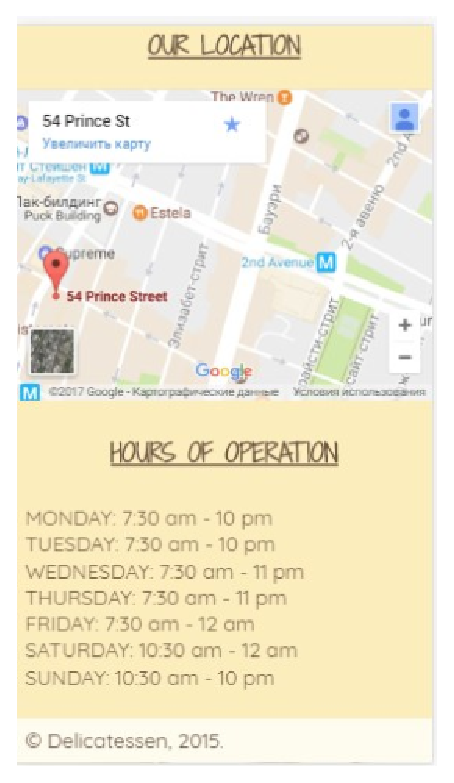
\includegraphics{images/76.eps}
\caption{Afisare Smartphone - Home}
\end{figure}

\begin{figure}[h]
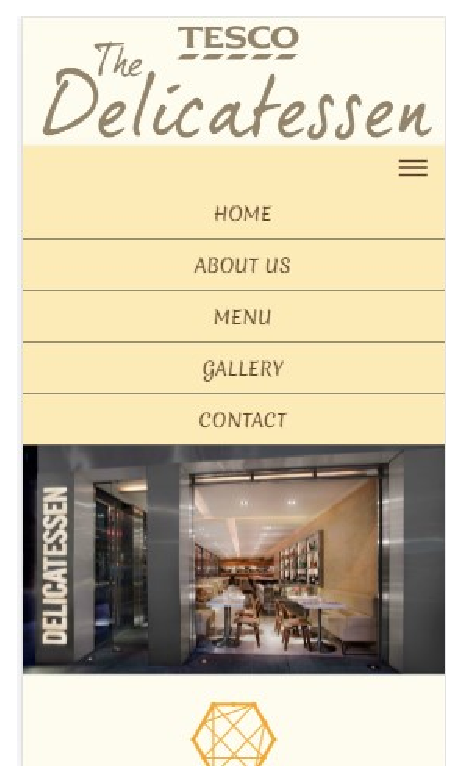
\includegraphics{images/77.eps}
\caption{Afisare Smartphone - Home}
\end{figure}

\begin{figure}[h]

\includegraphics{images/8.eps}
\caption{Afisare Smartphone - About Us}
\end{figure}

\begin{figure}[h]
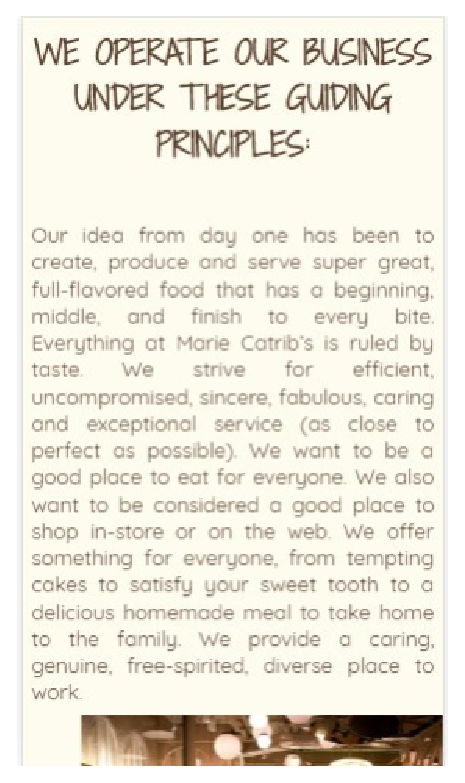
\includegraphics{images/81.eps}
\caption{Afisare Smartphone - About Us}
\end{figure}

\begin{figure}[h]
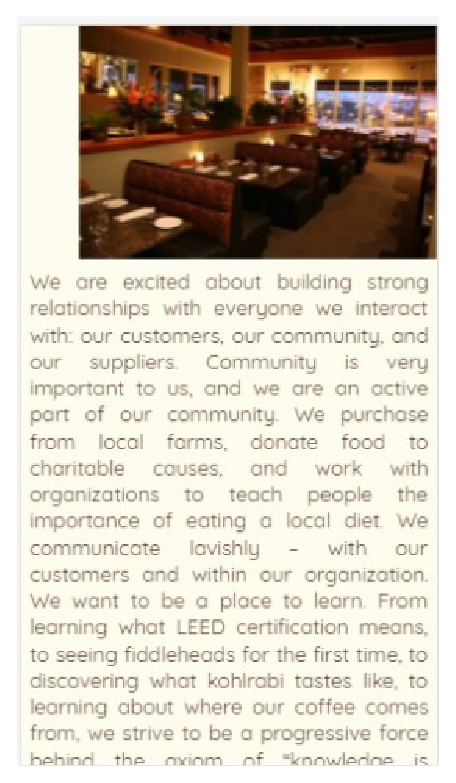
\includegraphics{images/82.eps}
\caption{Afisare Smartphone - About Us}
\end{figure}

\begin{figure}[h]
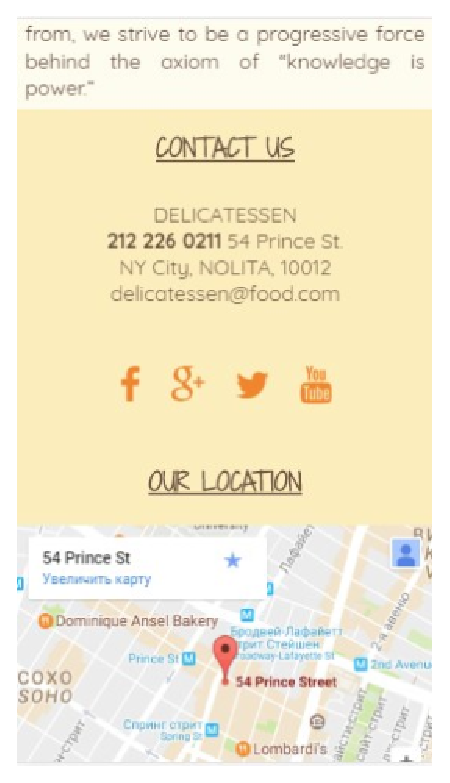
\includegraphics{images/83.eps}
\caption{Afisare Smartphone - About Us}
\end{figure}

\begin{figure}[h]
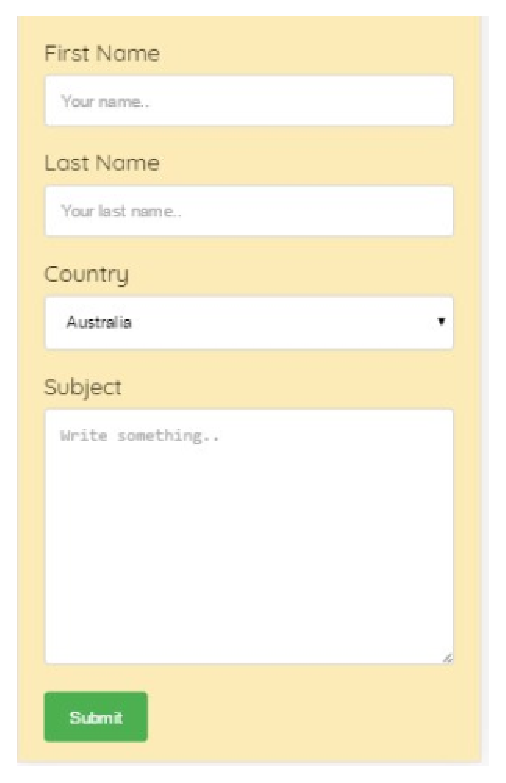
\includegraphics{images/9.eps}
\caption{Afisare Smartphone - Contact}
\end{figure}

\begin{figure}[h]
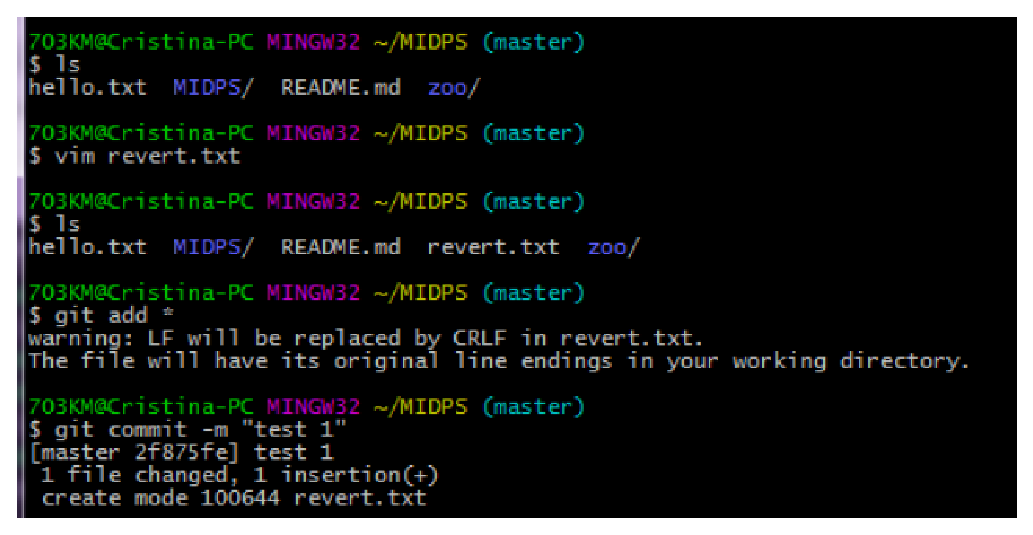
\includegraphics{images/10.eps}
\caption{Afisare Smartphone - Gallery}
\end{figure}

\begin{figure}[h]
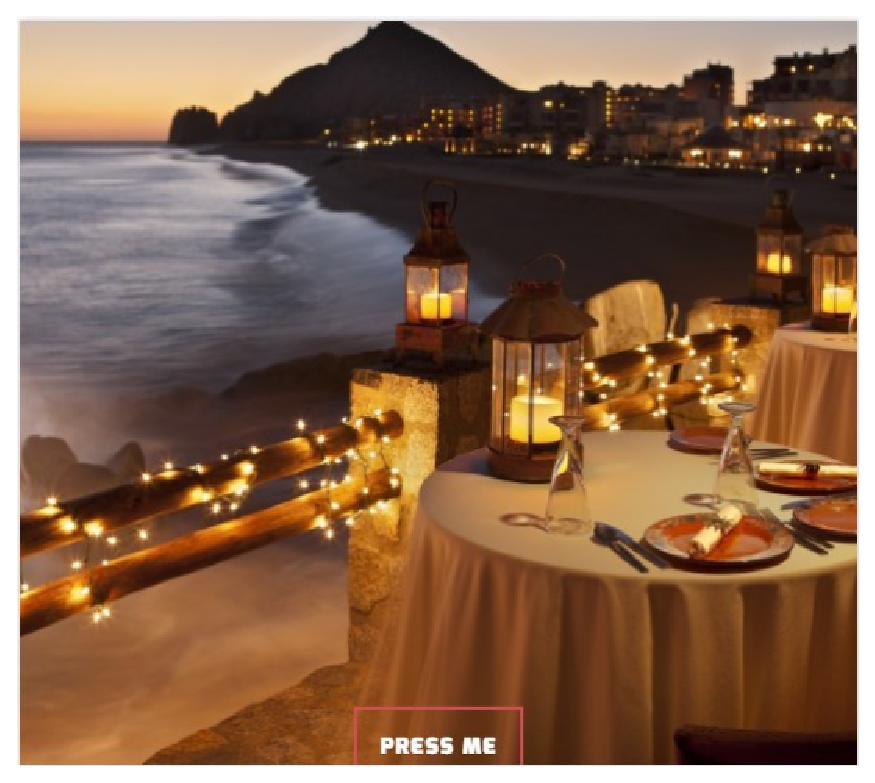
\includegraphics{images/11.eps}
\caption{Afisare Tablet - main}
\end{figure}

\begin{figure}[h]
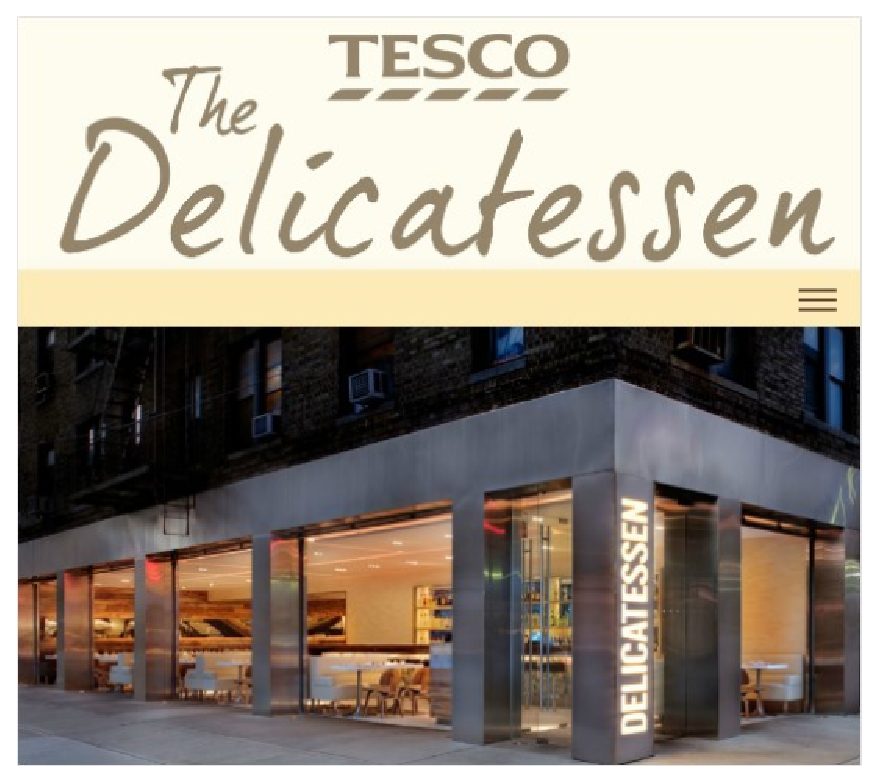
\includegraphics{images/12.eps}
\caption{Afisare Tablet - Home}
\end{figure}

\begin{figure}[h]
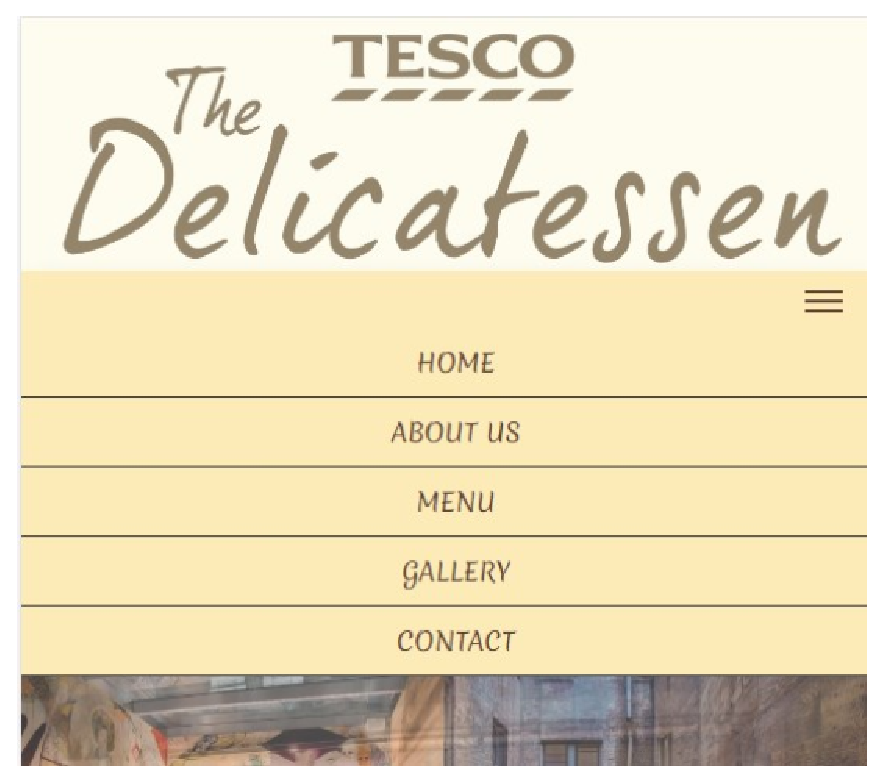
\includegraphics{images/121.eps}
\caption{Afisare Tablet - Home}
\end{figure}

\begin{figure}[h]
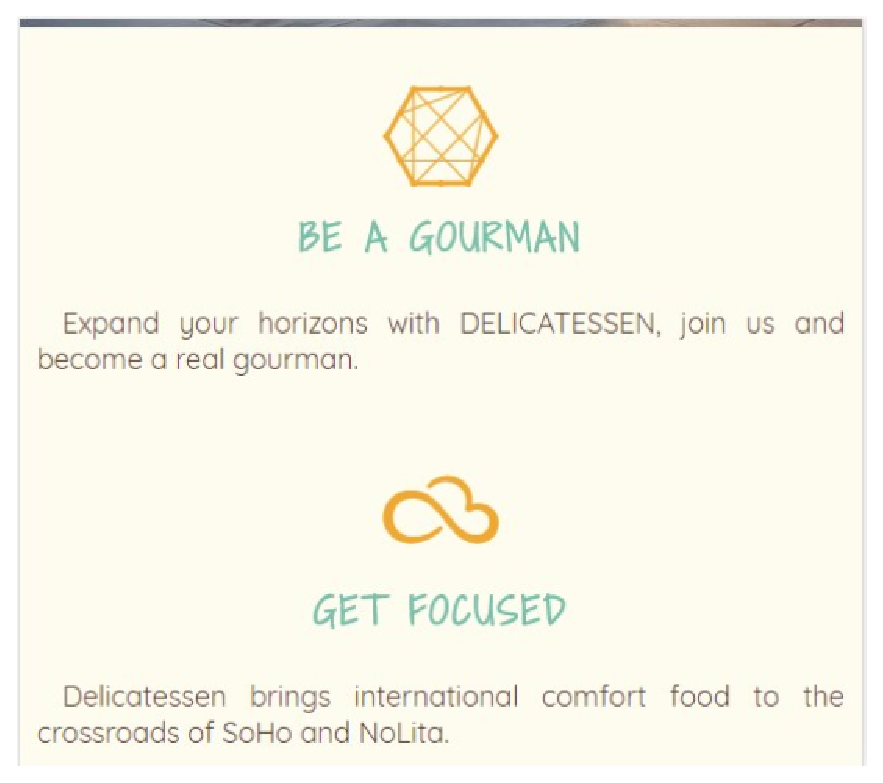
\includegraphics{images/122.eps}
\caption{Afisare Tablet - Home}
\end{figure}

\begin{figure}[h]
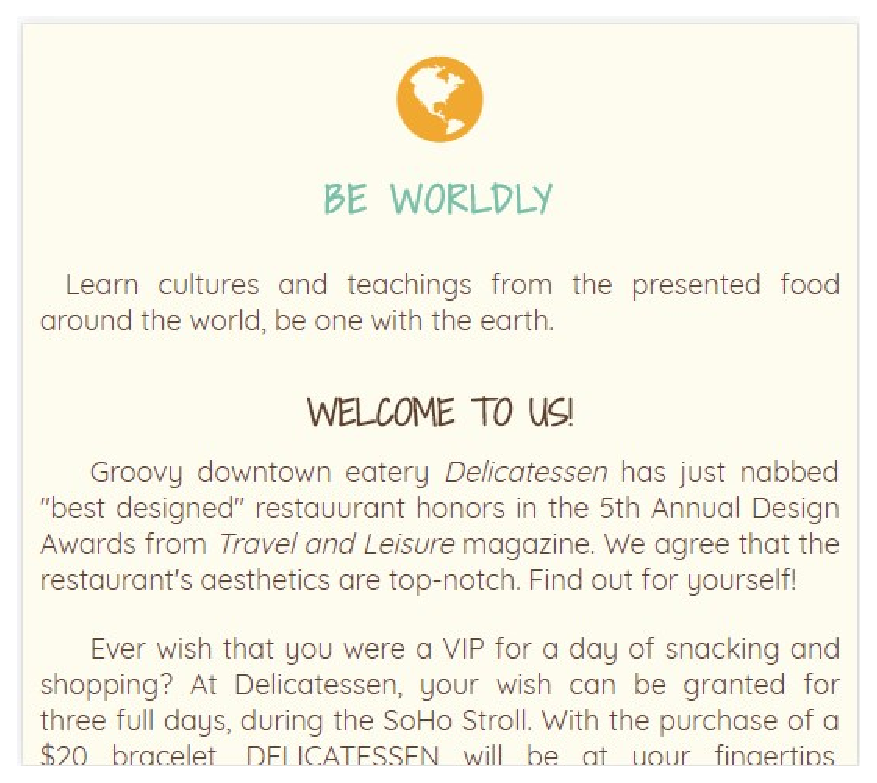
\includegraphics{images/123.eps}
\caption{Afisare Tablet - Home}
\end{figure}

\begin{figure}[h]
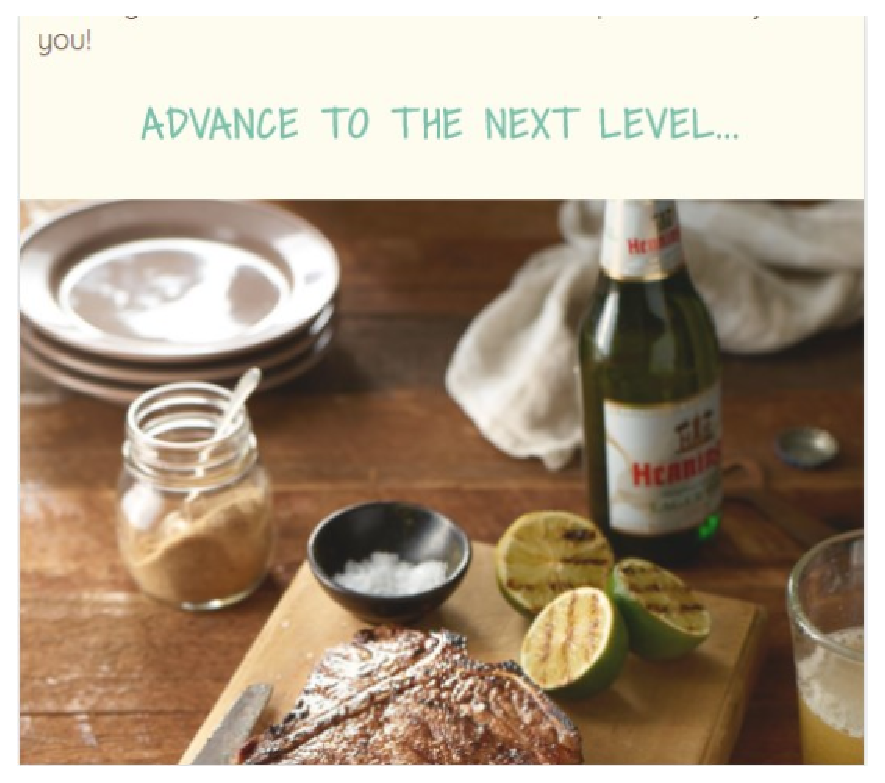
\includegraphics{images/124.eps}
\caption{Afisare Tablet - Home}
\end{figure}

\begin{figure}[h]
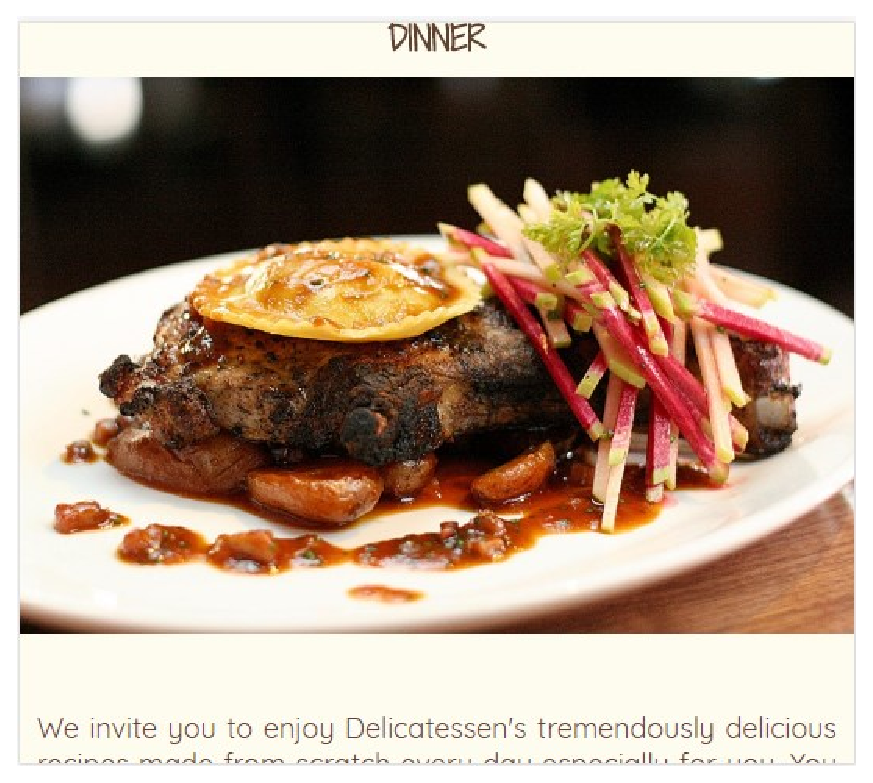
\includegraphics{images/125.eps}
\caption{Afisare Tablet - Home}
\end{figure}

\begin{figure}[h]
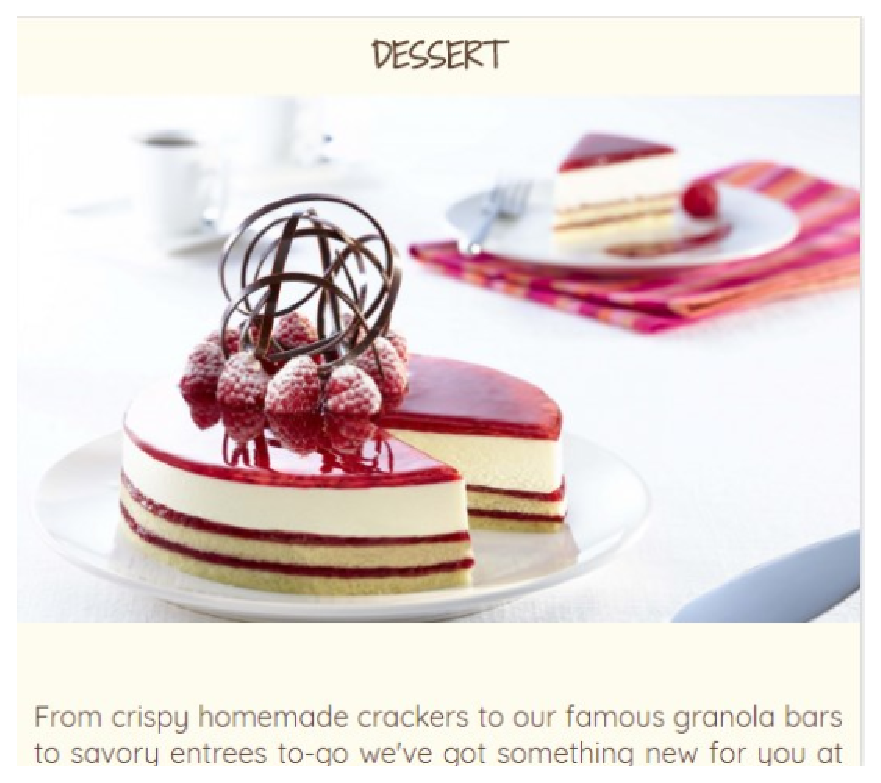
\includegraphics{images/126.eps}
\caption{Afisare Tablet - Home}
\end{figure}

\begin{figure}[h]
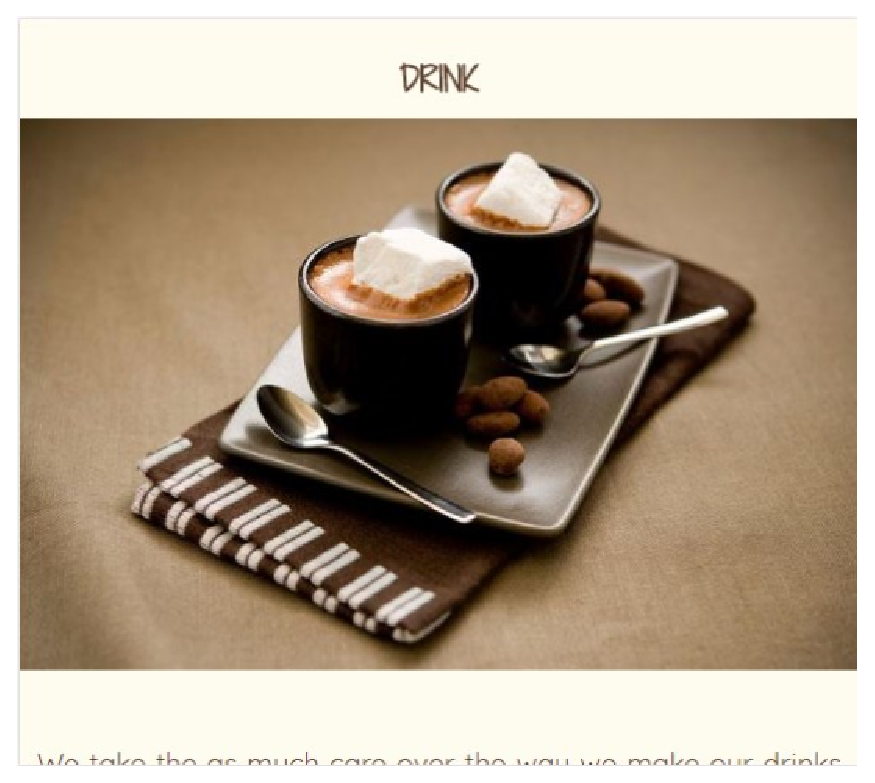
\includegraphics{images/127.eps}
\caption{Afisare Tablet - Home}
\end{figure}

\begin{figure}[h]

\includegraphics{images/128.eps}
\caption{Afisare Tablet - Home}
\end{figure}

\begin{figure}[h]
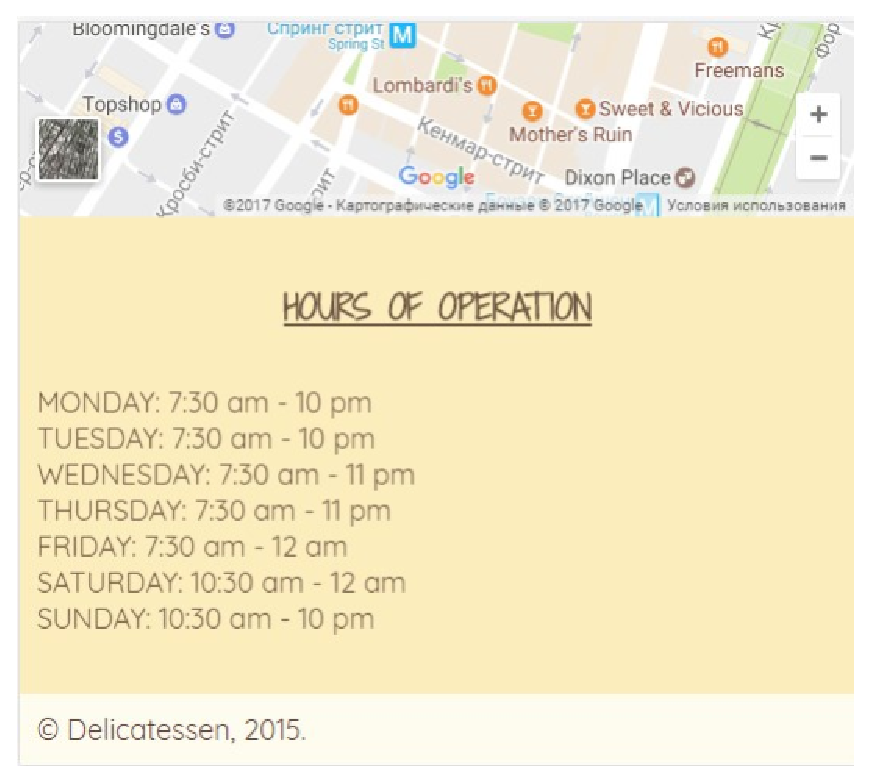
\includegraphics{images/129.eps}
\caption{Afisare Tablet - Home}
\end{figure}

\begin{figure}[h]
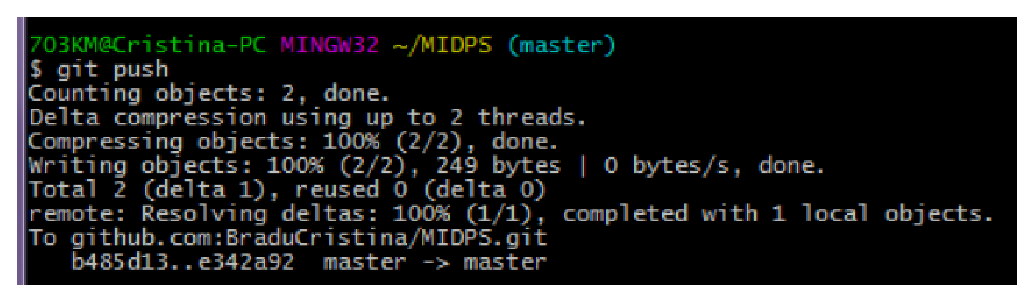
\includegraphics{images/13.eps}
\caption{Afisare Tablet - About Us}
\end{figure}

\begin{figure}[h]
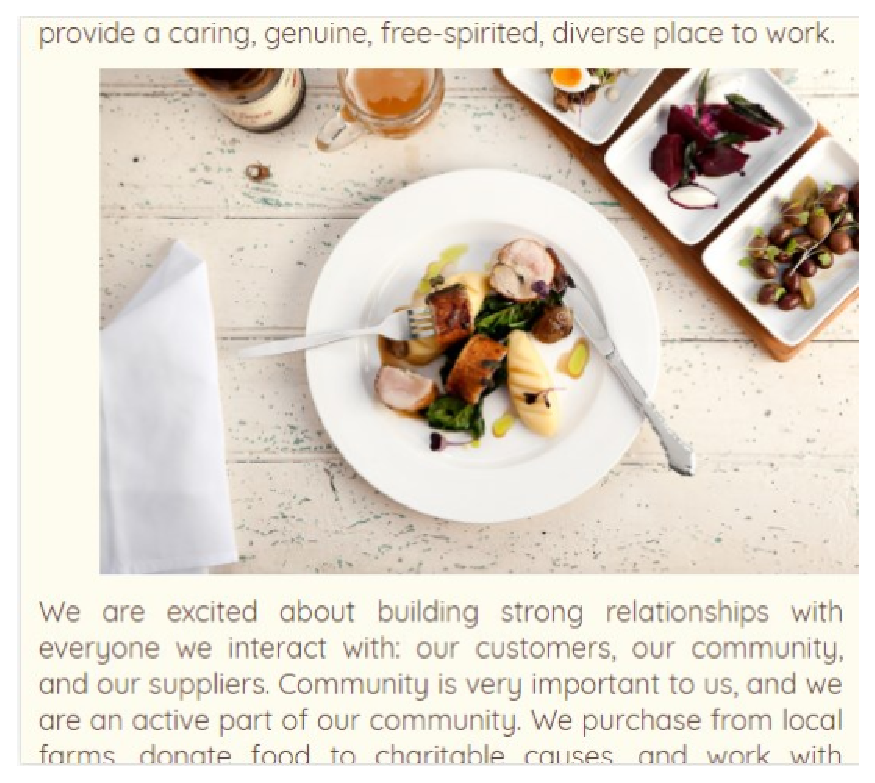
\includegraphics{images/131.eps}
\caption{Afisare Tablet - About Us}
\end{figure}

\begin{figure}[h]
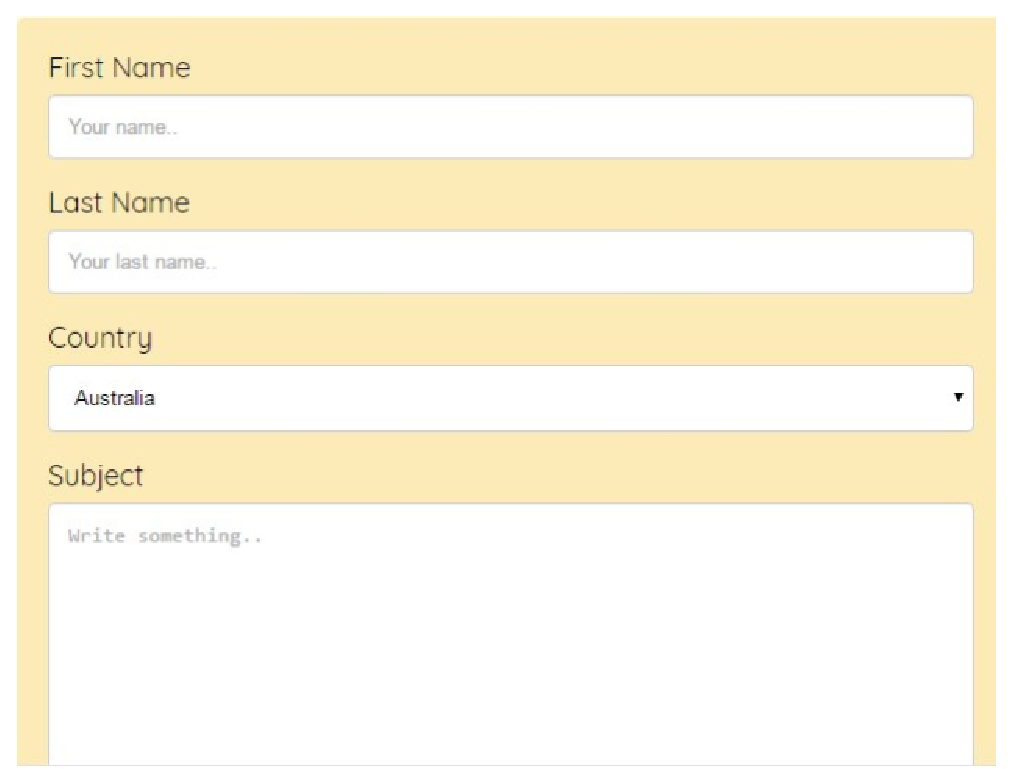
\includegraphics{images/14.eps}
\caption{Afisare Tablet - Contact}
\end{figure}

\begin{figure}[h]
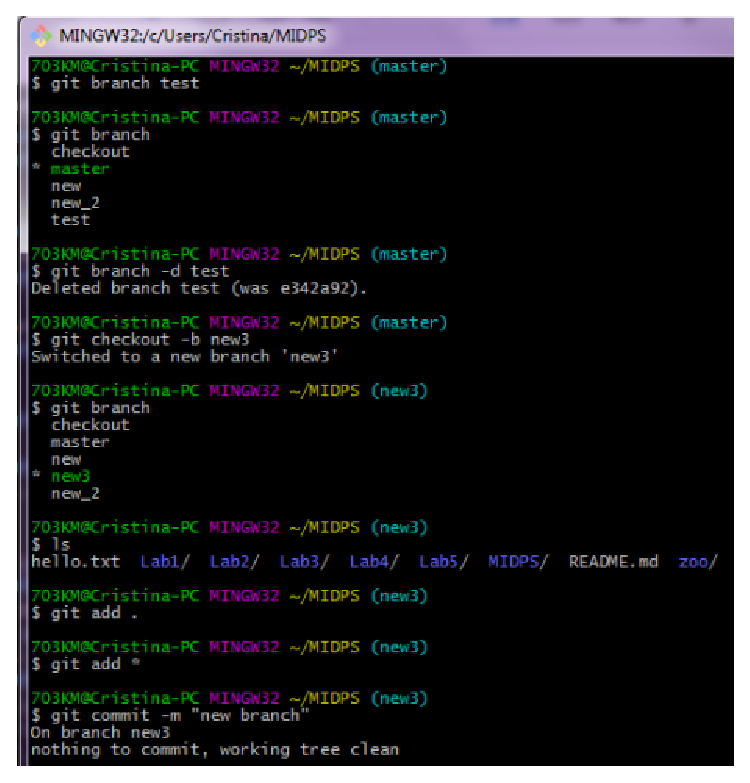
\includegraphics{images/15.eps}
\caption{Afisare Tablet - Gallery}
\end{figure}

\clearpage
\section*{Concluzie}

In lucrarea de laborator nr. 3 cu tema "Web Development", am implementat cunostintele obtinute in sfera data, studiind materiale suplimentare de pe YouTube, si alte site-uri specializate in cursuri online, precum Coursera. Mai devreme, am lucrat cu HTML/CSS si Javascript, si de aceea nu a fost complicat pentru mine sa efectuez front-endul site-ului prezent. Mi-a parut interesanta studierea altor tehnologii precum jquery sau AJAX, acestea permitindu-mi sa "oformez" paginile web mult mai placut vizibil, si user friendly. 
Am inceput sa lucrez si cu baze de date, initializind o forma pentru inregistrarea utilizatorilor. Pentru aceasta am apelat la MySQL, WAMP Server pentru localhost si desigur, am lucrat cu PhpMyAdmin.
Cunostintele obtinute cred ca le voi dezvolta cit mai mult posibil, pentru ca sfera data mi-a paraut destul de interesanta.
In concluzie pot afirma ca aptitudinile obtinute in urma efectuarii lucrarii de laborator date, si actualizindu-le zi de zi, imi vor prinde foarte bine in viitor, odata cu dezbvoltarea noilor tehnologii.

\clearpage

\end{document}